\documentclass[]{article}
\usepackage{lmodern}
\usepackage{amssymb,amsmath}
\usepackage{ifxetex,ifluatex}
\usepackage{fixltx2e} % provides \textsubscript
\ifnum 0\ifxetex 1\fi\ifluatex 1\fi=0 % if pdftex
  \usepackage[T1]{fontenc}
  \usepackage[utf8]{inputenc}
\else % if luatex or xelatex
  \ifxetex
    \usepackage{mathspec}
  \else
    \usepackage{fontspec}
  \fi
  \defaultfontfeatures{Ligatures=TeX,Scale=MatchLowercase}
\fi
% use upquote if available, for straight quotes in verbatim environments
\IfFileExists{upquote.sty}{\usepackage{upquote}}{}
% use microtype if available
\IfFileExists{microtype.sty}{%
\usepackage{microtype}
\UseMicrotypeSet[protrusion]{basicmath} % disable protrusion for tt fonts
}{}
\usepackage[margin=1in]{geometry}
\usepackage{hyperref}
\hypersetup{unicode=true,
            pdftitle={A DFT study to module a SiO2 messoporius surface},
            pdfauthor={Ciellie Jansen van Vuuren},
            pdfborder={0 0 0},
            breaklinks=true}
\urlstyle{same}  % don't use monospace font for urls
\usepackage{graphicx,grffile}
\makeatletter
\def\maxwidth{\ifdim\Gin@nat@width>\linewidth\linewidth\else\Gin@nat@width\fi}
\def\maxheight{\ifdim\Gin@nat@height>\textheight\textheight\else\Gin@nat@height\fi}
\makeatother
% Scale images if necessary, so that they will not overflow the page
% margins by default, and it is still possible to overwrite the defaults
% using explicit options in \includegraphics[width, height, ...]{}
\setkeys{Gin}{width=\maxwidth,height=\maxheight,keepaspectratio}
\IfFileExists{parskip.sty}{%
\usepackage{parskip}
}{% else
\setlength{\parindent}{0pt}
\setlength{\parskip}{6pt plus 2pt minus 1pt}
}
\setlength{\emergencystretch}{3em}  % prevent overfull lines
\providecommand{\tightlist}{%
  \setlength{\itemsep}{0pt}\setlength{\parskip}{0pt}}
\setcounter{secnumdepth}{0}
% Redefines (sub)paragraphs to behave more like sections
\ifx\paragraph\undefined\else
\let\oldparagraph\paragraph
\renewcommand{\paragraph}[1]{\oldparagraph{#1}\mbox{}}
\fi
\ifx\subparagraph\undefined\else
\let\oldsubparagraph\subparagraph
\renewcommand{\subparagraph}[1]{\oldsubparagraph{#1}\mbox{}}
\fi

%%% Use protect on footnotes to avoid problems with footnotes in titles
\let\rmarkdownfootnote\footnote%
\def\footnote{\protect\rmarkdownfootnote}

%%% Change title format to be more compact
\usepackage{titling}

% Create subtitle command for use in maketitle
\newcommand{\subtitle}[1]{
  \posttitle{
    \begin{center}\large#1\end{center}
    }
}

\setlength{\droptitle}{-2em}
  \title{A DFT study to module a SiO\textsubscript{2} messoporius surface}
  \pretitle{\vspace{\droptitle}\centering\huge}
  \posttitle{\par}
  \author{Ciellie Jansen van Vuuren}
  \preauthor{\centering\large\emph}
  \postauthor{\par}
  \predate{\centering\large\emph}
  \postdate{\par}
  \date{3/1/2018}

\usepackage{ragged2e}

\begin{document}
\maketitle

\hypertarget{abstract}{%
\subsection{Abstract}\label{abstract}}

Three \(\alpha\)-Quartz ,spacegroup 180, surfaces were modelled using
crystallographic data from pearson\ldots{}. obtained in the Medea
package database. Surface planes with miller indexes 100, 110 and 200
were cut from the bulk structure. The different surfaces were compared
to identify the ideal MCM-41 surface to be used as a catalyst support.

\hypertarget{introduction}{%
\section{Introduction}\label{introduction}}

The utilisation of homogeneos catalysts in industry are limited, due to
the fact that it is expensive to extract the catalyst from post-reaction
mixtures (Balcar \& Čejka, 2013)(Kotzé, 2015). Research especialy in the
pharmaseutlical and petrochemistry industries took an intrest in the
imobilisation or heteroganasion of a homgeneous catalyst as a posible
solution to the mentiond problem. Although the activity and selectivity
of heterogeneous catalytic reactions are lower than homogeneous
reactions, the advantage of separation, recovery and recycling outweigh
these shortcomings. It is however important to ensure that the
effectiveness of the immobilized homogeneous catalyst is not
dramatically compromised {[}7, 8{]}. Therefore the main objective in the
successful immobilization of homogeneous catalyst systems is to combine
the high activity and selectivity properties of homogeneous catalysts
with the ease of recovery of a heterogeneous catalyst. To accomplish
this the selection of an appropriate support material is very important
{[}7{]}.

Support materials can be divided into three categories e.g.~insoluble
organic, polymeric or inorganic supports. Immobilization by using
insoluble organic supports involves ultrafiltration techniques as seen
in the separation of the PUK-Grubbs 2 catalyst by using organic solvent
nanofiltration {[}8{]}. Van der Gryp et al. {[}8{]} performed this
separation using organic membranes and discovered that the catalyst can
be successfully separated, but its lifetime was dramatically decreased
during the filtration process {[}7, 8{]}. Polymer supports on the other
hand provide easier filtration techniques; multiple coordination sites
and the possibility to incorporate a molecular catalyst into the polymer
structure. These are great advantages, but during the filtration process
the thermal stability remains low {[}7{]}. Inorganic supports have a
high thermal stability, it provides for multiple coordination sites
because it contains a large surface area (BET), big pores and narrow
pore size distributions. Therefore inorganic supports are more effective
in the immobilization of homogeneous catalysts systems than organic or
polymeric support surfaces.{[}6{]}

There are three types of inorganic supports available, which is
categorized by their pore sizes and physical compositions:

\begin{enumerate}
\def\labelenumi{\arabic{enumi}.}
\tightlist
\item
  Inorganic microporous support materials have pore sizes \textless{}
  2nm, e.g.~Zeolites, Metal-Organic Frameworks (MOFs);
\item
  Inorganic mesoporous support materials have pore sizes in the range of
  2-15 nm, e.g.~MCM-41, SBA-15 and Aerogels; and
\item
  Inorganic macroporous support materials have pore sizes greater than
  50 nm, e.g.~glasses. {[}6, 7{]}
\end{enumerate}

Although microporous and macroporious support materials have the ability
to be used as heterogeneous support, it doesn't have an industrial
appeal yet {[}6, 7{]}. Therefore the focus is on mesoporous support
materials. Since the successful synthesis of mesoporous materials by
Mobil in 1992, the research field in using and synthesizing mesoporious
materials as support materials for heterogeneous catalytic reactions has
grown significantly. Mesoporous silicates have a periodic structure,
although the walls are not crystalline. The original synthesis of
mesoporous support material was defined as the M41S family containing
hexagonal MCM-41, cubic MCM-48 and lamellar MCM-50 structures. A more
visual representation of the different structures can be seen in Figure
1

\begin{center}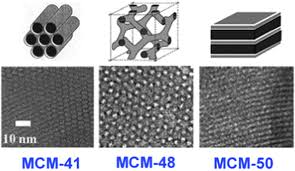
\includegraphics[width=0.9\linewidth]{Data/Images/Mcm-structures} \end{center}

Figure 1: Different structures of the M41S family.{[}9{]}(Izumi \emph{et
al.}, 2004)

Unfortunately M41S materials have a limitation in pore diameter,
approximately 80 Å; which affects the separation of large molecules
{[}10{]}. Zhao et al. {[}11{]} extended the family of inorganic
mesoporous support materials by synthesizing Santa Barbara Amorphous
(SBA) type materials, with a pore diameter ranging between 20 to 300 Å.

The surface of mesoporous support materials contain accessible hydroxyl
groups. This makes immobilization of homogeneous complexes on the silica
surface possible {[}7{]}. The crusial factor for immobilization of a
catalyst on the silica surface is the concentration, distribution and
accessibility of the silanol groups on the silica surface {[}6{]}.
Ramírez et al. {[}12{]} showed that the types of silanols present on the
silica surface are single, hydrogen bonded or germinal silanol groups as
shown in Figure 2.

\begin{center}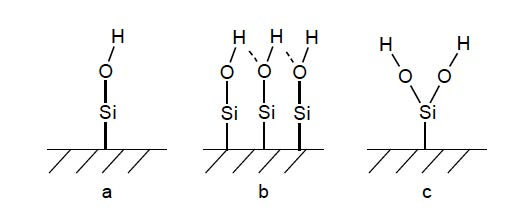
\includegraphics[width=0.9\linewidth]{Data/Images/Silanol_groups} \end{center}

Figure 2: Different silanol groups on the surface of a silica support:
(a) single, (b) hydrogen bonded and (c) geminal silanol
groups{[}12{]}(Izumi \emph{et al.}, 2004)

Coordination of the metal complexes to the support can either take place
by binding of the metal ions directly or via organic molecule linkers to
the silanols. Sels and co-workers {[}13{]} observed that a weak physical
interaction between a neutral Hoveyda-Grubbs- II type complex and the
inorganic support was enough to seperate the complex from the mixture
and altered surfaces using linkers was not nessesary. Cabrera et al.
{[}14{]} and Schachner et al. {[}15{]} also found that ruthenium-based
metathesis catalysts containing a hemilabile pyridine-alkoxide ligand
adsorb extremely well onto an unmodified silica support without
compromising too much on the homogeneous catalytic effectiveness.

\hypertarget{experimental}{%
\section{Experimental}\label{experimental}}

\hypertarget{results-and-discussion}{%
\section*{Results and discussion}\label{results-and-discussion}}
\addcontentsline{toc}{section}{Results and discussion}

\hypertarget{refs}{}
\leavevmode\hypertarget{ref-RN44}{}%
Balcar, H. \& Čejka, J. 2013. Mesoporous molecular sieves as advanced
supports for olefin metathesis catalysts. \emph{Coordination Chemistry
Reviews}. 257(21-22):3107--3124.

\leavevmode\hypertarget{ref-RN96}{}%
Izumi, S., Hara, S., Kumagai, T., \& Sakai, S. 2004. Classification of
amorphous-silicon microstructures by structural parameters: Molecular
dynamics study. \emph{Computational Materials Science}.
31(3-4):258--268.

\leavevmode\hypertarget{ref-RN90}{}%
Kotzé, H. de V. 2015. Immobilized ru(II) catalysts for transfer
hydrogenation and oxidative alkene cleavage reactions (Journal Article).
Stellenbosh University South Africa.


\end{document}
